\documentclass{article}
\usepackage[margin=1.25in]{geometry}
\usepackage{amsmath, amssymb, setspace, enumerate, enumitem}
\usepackage{setspace}
\usepackage{graphicx}
\onehalfspacing

\begin{document}
    \begin{enumerate}
        \item \begin{enumerate}[label=(\alph*)]
            \item For the input point [2,1] and y = -1, with weights 0.15 applied. For identity: The first layer returns with results [ [0.2778125  0.2778125] [0.13890625 0.13890625] ] and layer two returns with results [[0.47529864] [0.47529864]]. For tanh: first layer w1: [[0.27569254 0.27569254][0.13784627 0.13784627]], second layer [[0.47167168][0.47167168]]. The $E_{in}(w)$ obtained was $0.3172898231266975$
            \item After peturbing the weights, I achieved the following: identity w1: [[0.27796641 0.27796641]
            [0.1389832  0.1389832 ]]
           w2: [[0.47564328]
            [0.47564328]] and tanh: w1: [[0.2758401  0.2758401 ]
            [0.13792005 0.13792005]]
           w2: [[0.47200485]
            [0.47200485]]. $E_{in}(w)$ was 0.31737905364130986\\[0.25in]
            As stated by the hint, after peturbing the weights, the results were relatively similar, only different in the final few digits, therefore we can conclude that our algorithm is correct.
        \end{enumerate}
        \item \begin{enumerate}
            \item After running for $2 \times 10^6$ iterations, the following $E_{in}$ versus iterations graph was created:\\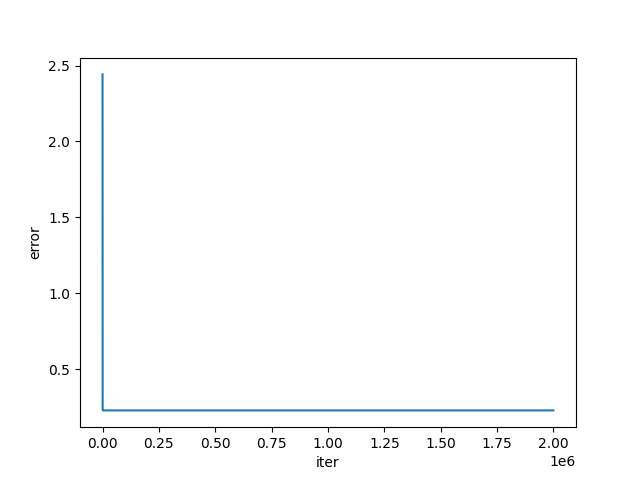
\includegraphics[scale=0.5]{images/2a1.png}\\
            Since it seems difficult to infer the values, I decided to rerun the algorithm with a lower iterations for $iter = 1000$, this was the graph that it plotted:\\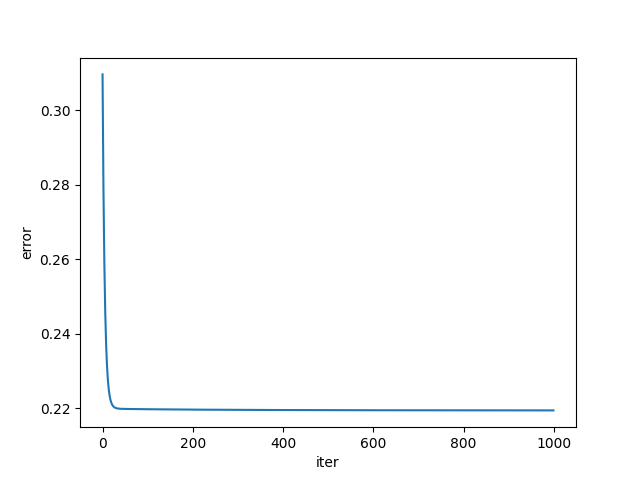
\includegraphics[scale=0.5]{images/2a2.png}\\
            It seems to converge pretty quickly at $iterations \approx 10$\\
            I believe that I did something wrong for this neural network to classify the digits because it seems like the decision region is incorrect... However, I added it regardless to show work:\\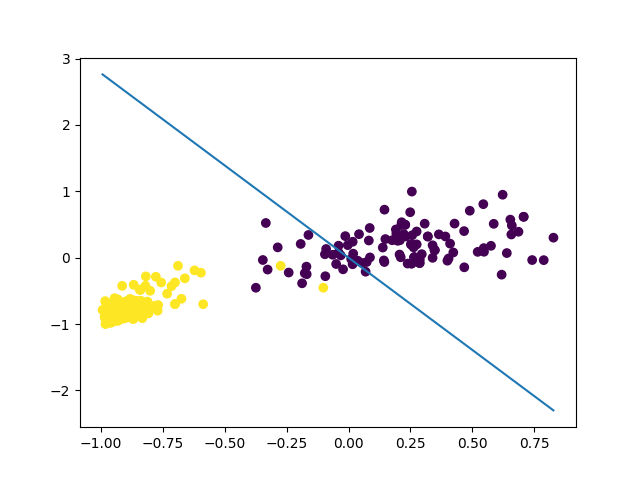
\includegraphics[scale=0.5]{images/2a3.png}\\This achieved a $E_{in} = 0.266$, pretty high for the neural network, I was expecting lower.
            \item Since my algorithm was wrong :(, I decided to focus on the other parts of the homework, it's unfortunately that I couldn't get the algorithm working. However, for the \textbf{Why divide iteration \# by N}, I believe it is to adjust the learning rate over time.
            \item omit
            \item omit
        \end{enumerate}
        \item \begin{enumerate}[label=(\alph*)]
            \item We're given two two-dimensional inputs, $x_1 = (1,0)$ and $x_2 = (-1,0)$. The optimal separating hyperplane is simply a line. For SVM, we want to find the separator that maximizes the margin. Both of these lines depict a horizontal line with slope 0, the perpendicular bisector is the negative reciprocal of the line, which is a vertical line. A vertical line in $x = 0$ is our solution.
            \item \begin{enumerate}[label=(\roman*)]
                \item They are the same point $z_1 = (1,0)$ and $z_2 = (-1,0)$
                \item The same, $z = 0$ and it's a vertical line.
            \end{enumerate}
            \item 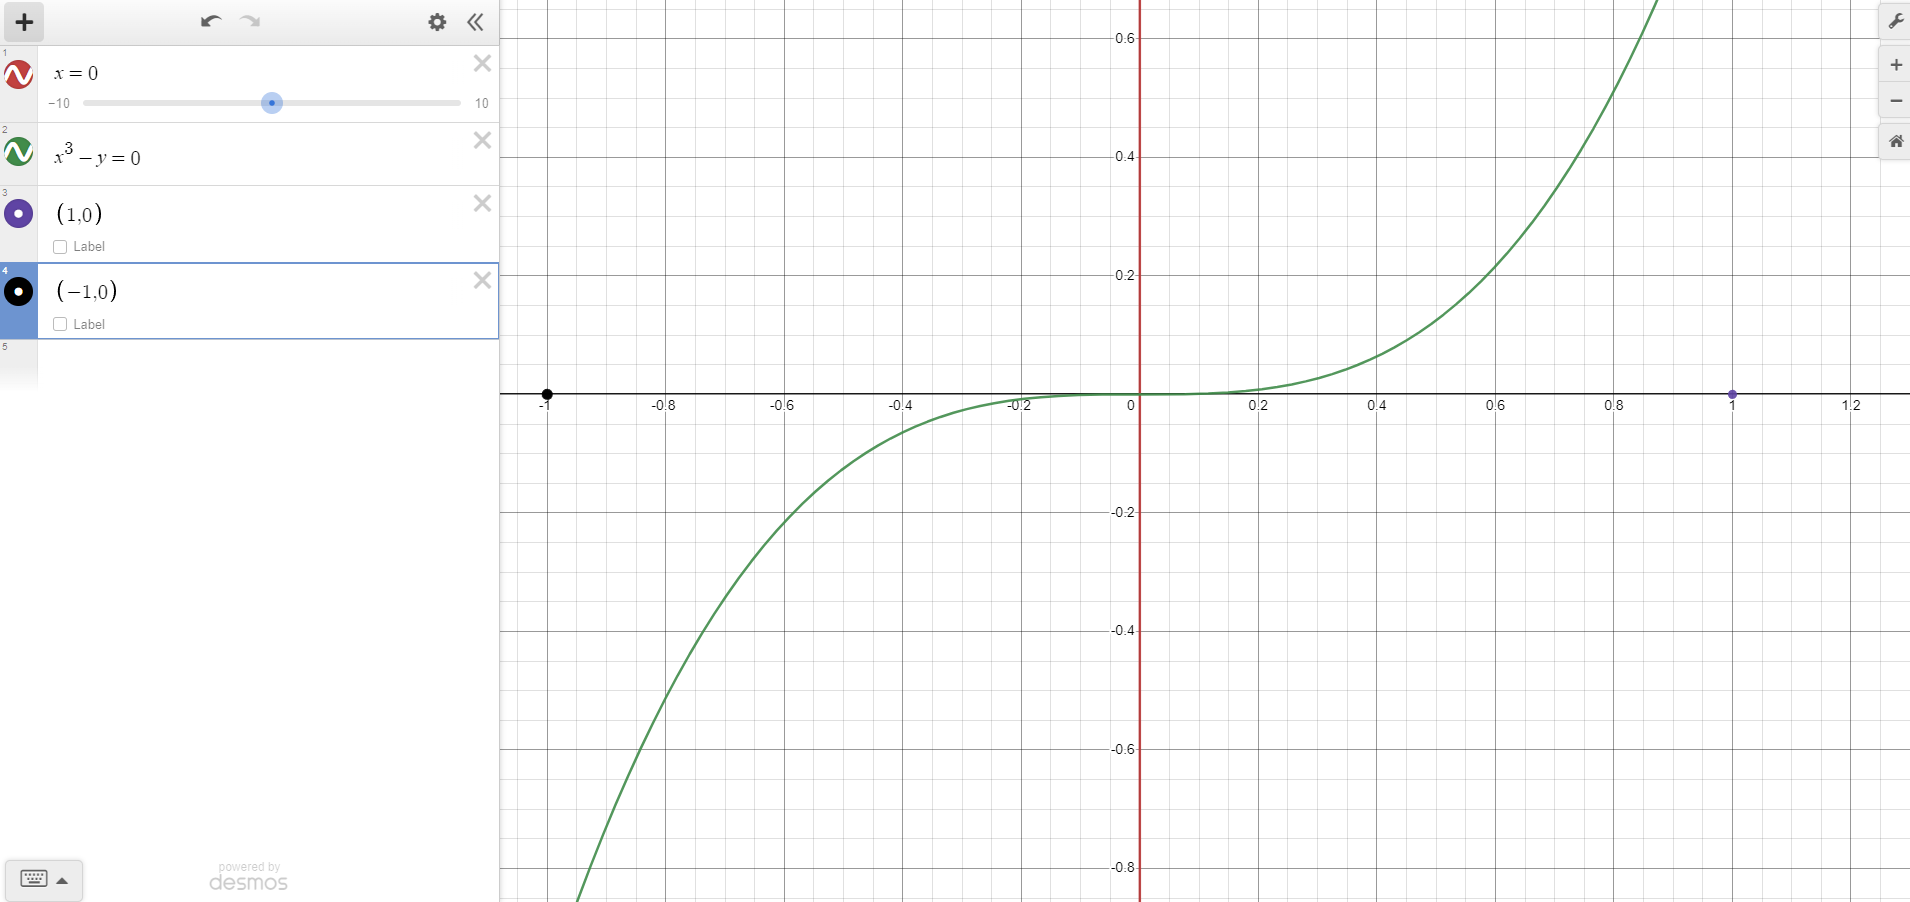
\includegraphics[scale=0.25]{images/3c.png}
            \item For $z(x) = \begin{bmatrix}
                    x^3_1 - x_2\\
                    x_1x_2
                \end{bmatrix}$, and $z(y) = \begin{bmatrix}
                    y^3_1 - y_2\\
                    y_1y_2
                \end{bmatrix}$, we can derive the following:
                \begin{align*}
                    K(x,y) &= z(x) \cdot z(y)\\
                    &= (x^3_1 - x_2)(y^3_1 - y_2) + (x_1x_2)(y_1y_2)\\
                    &= x^3_1y^3_1 - x^3_1y_2 - x_2y^3_1 + x_2y_2 + x_1x_2y_1y_2\\
                \end{align*}
            \item $h(x) = \text{sign}(x^3_1 - x_2 + x_1x_2)$
        \end{enumerate}
    \item \begin{enumerate}[label=(\alph*)]
        \item For small $C$, the value $C = 0.01$ was chosen, the following plot was generated with the plotted decision regions:\\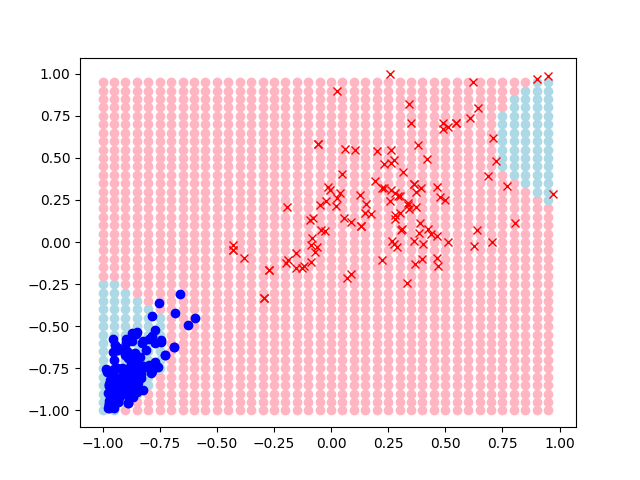
\includegraphics[scale=0.5]{images/4aregsmall.png}
        \\ For large $C$, the value $C = 10$ was chosen, the decision boundary was:\\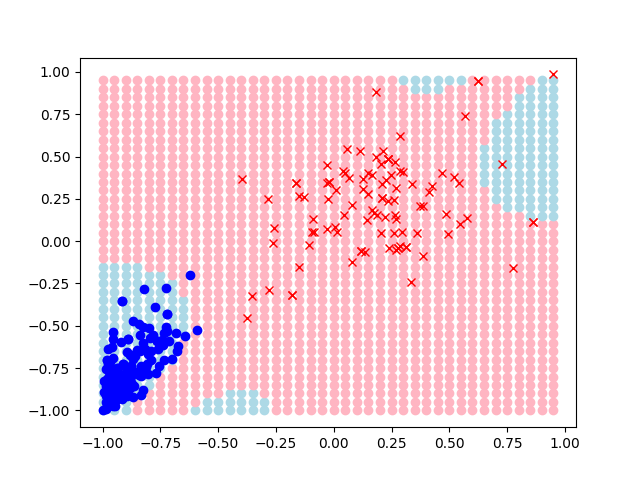
\includegraphics[scale=0.5]{images/4reglarge.png}
        \item For a small $C$, the complexity was low, we see more of less balanced regions of blues and reds for the decision boundary. When increasing the complexity, we see that the reds in the center have a smaller margin, meaning that the decision boundaries are more complex as also seen by the small bulbs of blue appearing on the sides.
        \item After running $C$ from $0.01$ to $10$, the lowest $C$ achieved was at $C = 1.77$, it had a $E_{test} = 0.031738$, the following decision boundary is plotted with the validation set data:\\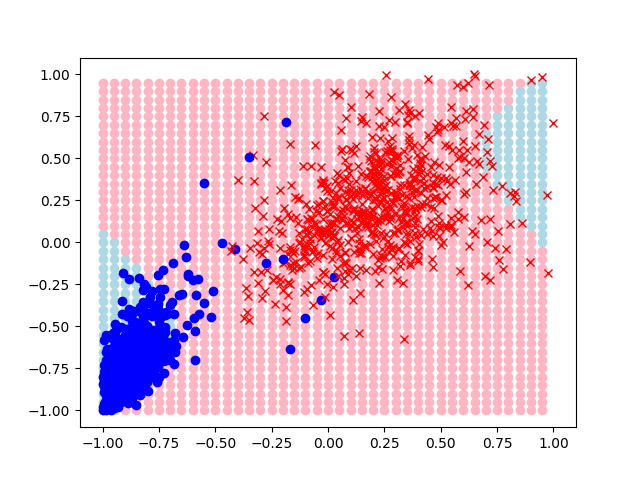
\includegraphics[scale=0.5]{images/4c.png}
    \end{enumerate}
    \end{enumerate}
\end{document}